\documentclass[11pt,preprint]{elsarticle}

\usepackage{lmodern}
%%%% My spacing
\usepackage{setspace}
\setstretch{1.2}
\DeclareMathSizes{12}{14}{10}{10}

% Wrap around which gives all figures included the [H] command, or places it "here". This can be tedious to code in Rmarkdown.
\usepackage{float}
\let\origfigure\figure
\let\endorigfigure\endfigure
\renewenvironment{figure}[1][2] {
    \expandafter\origfigure\expandafter[H]
} {
    \endorigfigure
}

\let\origtable\table
\let\endorigtable\endtable
\renewenvironment{table}[1][2] {
    \expandafter\origtable\expandafter[H]
} {
    \endorigtable
}


\usepackage{ifxetex,ifluatex}
\usepackage{fixltx2e} % provides \textsubscript
\ifnum 0\ifxetex 1\fi\ifluatex 1\fi=0 % if pdftex
  \usepackage[T1]{fontenc}
  \usepackage[utf8]{inputenc}
\else % if luatex or xelatex
  \ifxetex
    \usepackage{mathspec}
    \usepackage{xltxtra,xunicode}
  \else
    \usepackage{fontspec}
  \fi
  \defaultfontfeatures{Mapping=tex-text,Scale=MatchLowercase}
  \newcommand{\euro}{€}
\fi

\usepackage{amssymb, amsmath, amsthm, amsfonts}

\def\bibsection{\section*{References}} %%% Make "References" appear before bibliography


\usepackage[numbers]{natbib}

\usepackage{longtable}
\usepackage[margin=2.3cm,bottom=2cm,top=2.5cm, includefoot]{geometry}
\usepackage{fancyhdr}
\usepackage[bottom, hang, flushmargin]{footmisc}
\usepackage{graphicx}
\numberwithin{equation}{section}
\numberwithin{figure}{section}
\numberwithin{table}{section}
\setlength{\parindent}{0cm}
\setlength{\parskip}{1.3ex plus 0.5ex minus 0.3ex}
\usepackage{textcomp}
\renewcommand{\headrulewidth}{0.2pt}
\renewcommand{\footrulewidth}{0.3pt}

\usepackage{array}
\newcolumntype{x}[1]{>{\centering\arraybackslash\hspace{0pt}}p{#1}}

%%%%  Remove the "preprint submitted to" part. Don't worry about this either, it just looks better without it:

 \def\tightlist{} % This allows for subbullets!

\usepackage{hyperref}
\hypersetup{breaklinks=true,
            bookmarks=true,
            colorlinks=true,
            citecolor=blue,
            urlcolor=blue,
            linkcolor=blue,
            pdfborder={0 0 0}}


% The following packages allow huxtable to work:
\usepackage{siunitx}
\usepackage{multirow}
\usepackage{hhline}
\usepackage{calc}
\usepackage{tabularx}
\usepackage{booktabs}
\usepackage{caption}


\newenvironment{columns}[1][]{}{}

\newenvironment{column}[1]{\begin{minipage}{#1}\ignorespaces}{%
\end{minipage}
\ifhmode\unskip\fi
\aftergroup\useignorespacesandallpars}

\def\useignorespacesandallpars#1\ignorespaces\fi{%
#1\fi\ignorespacesandallpars}

\makeatletter
\def\ignorespacesandallpars{%
  \@ifnextchar\par
    {\expandafter\ignorespacesandallpars\@gobble}%
    {}%
}
\makeatother


% definitions for citeproc citations
\NewDocumentCommand\citeproctext{}{}
\NewDocumentCommand\citeproc{mm}{%
\href{\#cite.\detokenize{#1}}{#2}\nocite{#1}}

\makeatletter
% allow citations to break across lines
\let\@cite@ofmt\@firstofone
% avoid brackets around text for \cite:
\def\@biblabel#1{}
\def\@cite#1#2{{#1\if@tempswa , #2\fi}}
\makeatother
\newlength{\cslhangindent}
\setlength{\cslhangindent}{1.5em}
\newlength{\csllabelwidth}
\setlength{\csllabelwidth}{3em}
\newenvironment{CSLReferences}[2] % #1 hanging-indent, #2 entry-spacing
{\begin{list}{}{%
	\setlength{\itemindent}{0pt}
	\setlength{\leftmargin}{0pt}
	\setlength{\parsep}{0pt}
	% turn on hanging indent if param 1 is 1
	\ifodd #1
	\setlength{\leftmargin}{\cslhangindent}
	\setlength{\itemindent}{-1\cslhangindent}
	\fi
	% set entry spacing
	\setlength{\itemsep}{#2\baselineskip}}}
{\end{list}}

\usepackage{calc}
\newcommand{\CSLBlock}[1]{\hfill\break\parbox[t]{\linewidth}{\strut\ignorespaces#1\strut}}
\newcommand{\CSLLeftMargin}[1]{\parbox[t]{\csllabelwidth}{\strut#1\strut}}
\newcommand{\CSLRightInline}[1]{\parbox[t]{\linewidth - \csllabelwidth}{\strut#1\strut}}
\newcommand{\CSLIndent}[1]{\hspace{\cslhangindent}#1}


\urlstyle{same}  % don't use monospace font for urls
\setlength{\parindent}{0pt}
\setlength{\parskip}{6pt plus 2pt minus 1pt}
\setlength{\emergencystretch}{3em}  % prevent overfull lines
\setcounter{secnumdepth}{5}

%%% Use protect on footnotes to avoid problems with footnotes in titles
\let\rmarkdownfootnote\footnote%
\def\footnote{\protect\rmarkdownfootnote}
\IfFileExists{upquote.sty}{\usepackage{upquote}}{}

%%% Include extra packages specified by user

%%% Hard setting column skips for reports - this ensures greater consistency and control over the length settings in the document.
%% page layout
%% paragraphs
\setlength{\baselineskip}{12pt plus 0pt minus 0pt}
\setlength{\parskip}{12pt plus 0pt minus 0pt}
\setlength{\parindent}{0pt plus 0pt minus 0pt}
%% floats
\setlength{\floatsep}{12pt plus 0 pt minus 0pt}
\setlength{\textfloatsep}{20pt plus 0pt minus 0pt}
\setlength{\intextsep}{14pt plus 0pt minus 0pt}
\setlength{\dbltextfloatsep}{20pt plus 0pt minus 0pt}
\setlength{\dblfloatsep}{14pt plus 0pt minus 0pt}
%% maths
\setlength{\abovedisplayskip}{12pt plus 0pt minus 0pt}
\setlength{\belowdisplayskip}{12pt plus 0pt minus 0pt}
%% lists
\setlength{\topsep}{10pt plus 0pt minus 0pt}
\setlength{\partopsep}{3pt plus 0pt minus 0pt}
\setlength{\itemsep}{5pt plus 0pt minus 0pt}
\setlength{\labelsep}{8mm plus 0mm minus 0mm}
\setlength{\parsep}{\the\parskip}
\setlength{\listparindent}{\the\parindent}
%% verbatim
\setlength{\fboxsep}{5pt plus 0pt minus 0pt}



\begin{document}



\begin{frontmatter}  %

\title{Baby Names}

% Set to FALSE if wanting to remove title (for submission)












\vspace{1cm}





\vspace{0.5cm}

\end{frontmatter}

\setcounter{footnote}{0}



%________________________
% Header and Footers
%%%%%%%%%%%%%%%%%%%%%%%%%%%%%%%%%
\pagestyle{fancy}
\chead{}
\rhead{}
\lfoot{}
\rfoot{\footnotesize Page \thepage}
\lhead{}
%\rfoot{\footnotesize Page \thepage } % "e.g. Page 2"
\cfoot{}

%\setlength\headheight{30pt}
%%%%%%%%%%%%%%%%%%%%%%%%%%%%%%%%%
%________________________

\headsep 35pt % So that header does not go over title




\section{\texorpdfstring{Baby name persistence
\label{Baby name persistence }}{Baby name persistence }}\label{baby-name-persistence}

First, I get the national names counts, or, the sum of each name across
all the states for each year and gender

Second, I rank all the names by their count (rank 1 being the most
popular), within each year-gender pairing.

Third, I create a function for the top n ranked names for year-gender
pairings

Fourth, in order to measure persistence, I tracked each each years top
25 names (male and female), and then checked where they ranked 1, 2 and
3 years later.The Spearman rank correlation is used, where a rank close
to 1 means the names stayed in the same order, and close to 0 means they
changed significantly.

Fifth, I plot the correlation over time.

\begin{figure}[H]

{\centering 
\includegraphics{22921893Question2_files/figure-latex/unnamed-chunk-5-1} 

}

\caption{The Persistence of Baby Names.}\label{fig:unnamed-chunk-5}
\end{figure}

The plot does indicate that the agencies suspicions may have been
correct, as there does appear to be a drop-off in persistence of the top
25 names from around 1990. The following table further confirms the
agencies suspicion. At each lag, the mean correlation drops from the
pre- to post-1990 period. This is possibly attributable to cultural
influences such as social media and streaming causing more frequent
waves of popular names. This motivates the subsequent section, which
investigates drivers of baby names.

\begin{longtable}[]{@{}lrr@{}}
\caption{Mean Correlation around 1990}\tabularnewline
\toprule\noalign{}
Period & Lag (years) & Mean Correlation \\
\midrule\noalign{}
\endfirsthead
\toprule\noalign{}
Period & Lag (years) & Mean Correlation \\
\midrule\noalign{}
\endhead
\bottomrule\noalign{}
\endlastfoot
Post 1990 & 1 & 0.944 \\
Pre 1990 & 1 & 0.966 \\
Post 1990 & 2 & 0.879 \\
Pre 1990 & 2 & 0.929 \\
Post 1990 & 3 & 0.825 \\
Pre 1990 & 3 & 0.893 \\
\end{longtable}

\section{\texorpdfstring{Investigating naming spikes
\label{Investigating naming spikes }}{Investigating naming spikes }}\label{investigating-naming-spikes}

First, I check the distribution of the data in order to get a threshold
which will be use to filter out low-volume names. 500 is chosen as the
threshold.

Then, I calculate the naming spikes as year-on-year percentage changes.

\begin{longtable}[]{@{}llrrr@{}}
\caption{Top 10 Year-on-Year Baby Name Spikes}\tabularnewline
\toprule\noalign{}
Name & Gender & Year & Count & \% Change \\
\midrule\noalign{}
\endfirsthead
\toprule\noalign{}
Name & Gender & Year & Count & \% Change \\
\midrule\noalign{}
\endhead
\bottomrule\noalign{}
\endlastfoot
Deneen & F & 1964 & 1572 & 31340 \\
Aaliyah & F & 1994 & 1412 & 28140 \\
Mallory & F & 1983 & 658 & 13060 \\
Tenley & F & 2010 & 650 & 12900 \\
Tammie & F & 1957 & 584 & 11580 \\
Jalen & M & 1992 & 583 & 9617 \\
Cataleya & F & 2012 & 616 & 7600 \\
Elian & M & 2000 & 542 & 5922 \\
Deanna & F & 1937 & 1605 & 5632 \\
Katina & F & 1972 & 2726 & 5579 \\
\end{longtable}

While a number of names are likely candidates for being driven by
pop-culture influence, the name Aaliyah has the 2nd largest year-on-year
spike, with a percentage change of 28 140 in 1994. As the following
search indicates, the pop singer Aaliyah's first entry into the
Billboard top 100 chart was also in 1994.

I create the following graph in order to visualise the spike in
popularity with and the rise of Aaliyah on the Billboard charts.

\begin{figure}[H]

{\centering 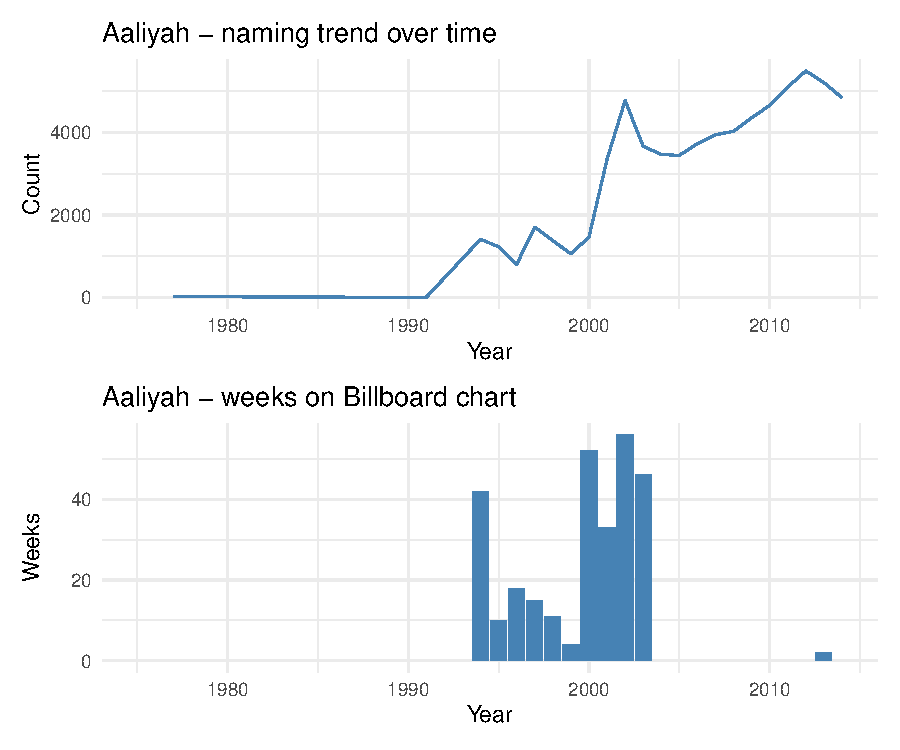
\includegraphics{22921893Question2_files/figure-latex/unnamed-chunk-10-1} 

}

\caption{The Name Aaliyah, Over Time.}\label{fig:unnamed-chunk-10}
\end{figure}

This indicates that pop-culture, fashionable trends, and celebrity
culture can influence naming trends over time.

\bibliography{Tex/ref}





\end{document}
